\section{Problem Statement and Research Hypothesis}
\label{sec:problem}

Let \(x\) denote a low-light image and \(y\) its paired sharp reference.
A restoration network \(F_\theta\) produces
\(\hat y=F_\theta(x)\). Conventional restoration training minimizes an
image-domain objective, while the intended downstream task may require
different visual representations for reliable object detection.

The central research question is:
\begin{quote}
Can task-aware low-light restoration improve downstream object-detection
performance while maintaining competitive restoration quality?
\end{quote}

The corresponding hypothesis is that direct detection-loss supervision
can guide DarkIR toward detection-relevant image structure more effectively
than an independent matched control. Balanced V2 tests this hypothesis by
adding a frozen ExDark-trained Faster R-CNN detection objective to a
matched restoration objective.

The study is not designed to claim that all low-light enhancement improves
detection. The original low-light inputs are retained as an important
baseline, and the final conclusion is based on measured changes relative
to V2-Control and absolute changes relative to the original inputs.

\section{Research Progression}
\label{sec:progression}

\subsection{Preliminary Project Report proposal}

The PPR proposed reproduction of DarkIR, verification of the published
LOLBlur benchmark, and a task-aware low-light restoration extension. It
introduced a generic task-loss formulation in which a fixed vision model
\(\phi(G(\cdot))\) compared intermediate features from restored and
reference images. The PPR also proposed adaptive feature modulation and a
four-way ablation separating task loss and modulation.

These proposals represent the original research plan. Adaptive feature
modulation and the B2/B3 ablation configurations were not implemented in
the completed experiments.

\subsection{Midterm V1 implementation}

The MTR documented V1, the first implemented task-aware method. V1 used
an L1 restoration term plus normalized cosine-distance consistency across
FPN features extracted by a frozen COCO-pretrained Faster R-CNN
ResNet-50 FPN:
\[
L_{\mathrm{V1}}
=
L_1
+
0.10L_{\mathrm{FPN}}.
\]

The detector parameters remained frozen. Reference features were computed
without gradients, while gradients through the restored-image branch
reached DarkIR. V1 used matched 50,000-step control and task-aware runs,
random 256-by-256 LOLBlur crops, AdamW, a \(10^{-5}\) to \(10^{-6}\)
learning-rate schedule, weight decay \(10^{-4}\), and seed 2026.

An initial implementation used manual detector normalization and did not
match torchvision's official detector transform. The corrected
implementation used the detector transform for both restored and reference
images. ExDark archive sidecars were excluded, annotations were corrected,
box formats were validated, detector score thresholding was configured,
and pycocotools COCOeval replaced the earlier custom matcher for final
reported metrics.

The matched V1 50,000-step results did not show a consistent detection
improvement over control, and the original low-light images remained
stronger under the frozen zero-shot detector. These observations supported
replacement of feature similarity with a direct detector-loss formulation.

\subsection{Balanced V2 redesign}

After V1, the method was redesigned to keep the restoration objective
matched in control and detection-guided arms. Both arms use L1, LPIPS,
and Sobel edge losses. The detection-guided arm adds the sum of Faster
R-CNN classification, box-regression, objectness, and RPN box-regression
losses from a frozen ExDark-trained teacher.

Balanced V2 uses 5,000 optimizer steps, a 600-image ExDark
detection-supervision partition, three detection weights, and two separate
detection evaluators. V1, 200-step pilots, 1K pilots, and 50K V1
checkpoints are retained as methodological history rather than final
results.

\section{Related Work}
\label{sec:related_work}

\subsection{Low-light image enhancement}

Traditional low-light enhancement methods learn mappings from
underexposed observations to normally exposed references. Chen
\etal~demonstrated direct RAW-to-RGB restoration for extreme low-light
scenes~\cite{chen2018learning}. Zero-DCE formulates enhancement as
image-specific curve estimation without paired reference
images~\cite{guo2020zero}. Decomposition-based approaches separate
low-light information into illumination and reflectance components or
low- and high-frequency representations~\cite{xu2020restore,uretinex2022}.
These approaches primarily optimize visual fidelity rather than the utility
of the enhanced image for a downstream computer vision task.

\subsection{DarkIR and low-light restoration}

DarkIR addresses low-light enhancement and motion blur jointly using an
asymmetric convolutional encoder-decoder with spatial and frequency-domain
processing~\cite{feijoo2025darkir}. Unlike transformer-based restoration
methods, DarkIR emphasizes efficient CNN components and compact model
configurations. In this project, DarkIR-m is used as the restoration
baseline because it provides a reproducible pretrained checkpoint and a
practical balance between model size and restoration performance.

\subsection{Downstream-aware low-light processing}

Several studies investigate the relationship between restoration quality
and downstream computer vision utility. Gu \etal proposed collaboration
between low-light enhancement and vision foundation models to improve both
visual and high-level performance~\cite{gu2025foundation}. Dark-ISP instead
introduces task-driven RAW-domain image processing for low-light object
detection~\cite{guo2025darkisp}. These studies demonstrate that low-level
enhancement and downstream detection can be optimized jointly, while also
showing that perceptual and task-level objectives may conflict.

\subsection{Object detection and ExDark}

Faster R-CNN performs object detection using a Region Proposal Network,
shared convolutional features, and class-specific box
prediction~\cite{ren2015fasterrcnn}. It is used here in two distinct roles:
as a frozen ExDark teacher for training and as an independent
COCO-pretrained evaluator~\cite{lin2014microsoft}. ExDark provides real low-light images annotated
with 12 object classes and bounding boxes~\cite{loh2019exdark}. Unlike a
synthetic degradation benchmark, ExDark contains naturally low-illumination
scenes and therefore provides a relevant downstream-detection evaluation
setting.

\subsection{Restoration and perception metrics}

PSNR and SSIM measure pixel or structural similarity~\cite{wang2004ssim},
while LPIPS uses deep feature representations to estimate perceptual
similarity~\cite{zhang2018lpips}. These metrics are useful for quantifying
restoration fidelity but do not directly measure detection utility. The
project consequently reports both LOLBlur restoration metrics and ExDark
object-detection metrics under controlled protocols.

\subsection{Extensions by this study}

Existing work motivates the use of restoration objectives and downstream
supervision, but does not determine whether a direct detection loss
improves a low-light-restoration network under a matched control. This
study adds a Balanced V2 comparison with:
\begin{itemize}
  \item identical L1, LPIPS, and edge losses in both arms;
  \item a frozen ExDark-trained detector as the task teacher;
  \item direct classification, box, objectness, and RPN-loss guidance;
  \item three detection-loss weights;
  \item separate ExDark-trained-teacher and independent-COCO evaluations;
  \item honest reporting of restoration--detection trade-offs and negative
  findings.
\end{itemize}

The V1 feature-consistency experiment is treated as prior methodological
history. Its FPN cosine-distance loss did not produce a consistent
detection improvement and was replaced by direct detection-loss supervision
in Balanced V2.

\section{Balanced V2 Methodology}
\label{sec:method}

\subsection{DarkIR baseline}

The restoration model is DarkIR-m with RGB input and output, width 32,
two middle encoder blocks, two middle decoder blocks, encoder block counts
\([1,2,3]\), decoder block counts \([3,1,1]\), dilations \([1,4,9]\), and
depthwise extra operations enabled. The model is initialized strictly from
the pretrained \texttt{models/DarkIR\_384.pt} checkpoint. Both final
Balanced V2 arms start from this checkpoint.

\begin{figure}[t]
\centering
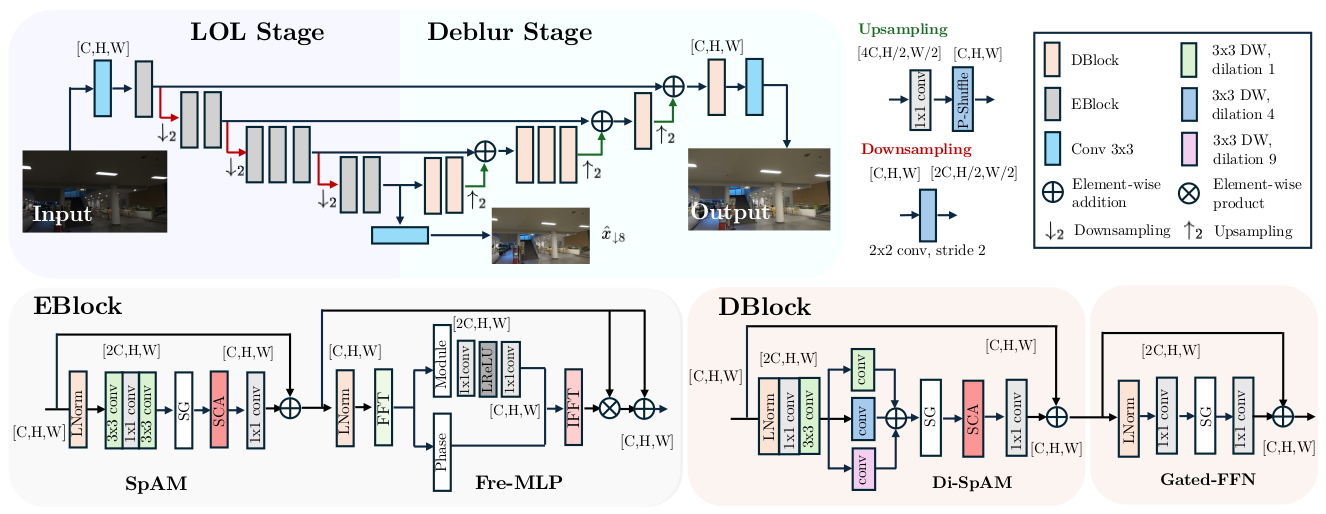
\includegraphics[width=\columnwidth]{fig/darkir_architecture.png}
\caption{DarkIR-m asymmetric encoder-decoder architecture used as the
restoration network in all final V2 arms; reproduced from DarkIR
\cite{feijoo2025darkir}.}
\label{fig:darkir_architecture}
\end{figure}

\section{ExDark Teacher Training}
\label{sec:exdark_teacher}

A separate 12-class Faster R-CNN ResNet-50 FPN teacher is trained to
support the Balanced V2 detection-loss objective. The detector is initialized
from torchvision COCO weights and modified to output 13 categories:
background plus the 12 ExDark classes. Matching COCO classification and
box-regression parameters are transferred to the corresponding ExDark
categories, while unmatched predictor rows remain initialized by the
replacement-head implementation.

The teacher training partition contains 2,099 ExDark images with 7,275
annotated boxes. The teacher-validation partition contains 300 images with
913 boxes. The partitions are disjoint from the 600-image detection-
supervision set and the 1,800-image official ExDark-validation set.

Teacher training uses 15 epochs, batch size 2, four data-loader workers,
AMP when enabled, backbone learning rate \(5\times10^{-4}\), head learning
rate \(2.5\times10^{-3}\), weight decay \(5\times10^{-4}\), momentum
0.9, and seed 2026. Multistep learning-rate milestones are placed at
approximately 60\% and 82\% of training. Horizontal-image augmentation is
used for the teacher-training data.

The best checkpoint is selected using teacher-validation mAP@50:95. At
epoch 15, the teacher achieves mAP@50 0.8189, mAP@50:95 0.5035, and
mAP@75 0.5452 on the 300-image teacher-validation partition. The resulting
checkpoint is \texttt{models/exdark\_teacher\_v2/best.pt}.

The teacher is not jointly fine-tuned with DarkIR during Balanced V2.
Its parameters remain frozen, and it supplies only the four Faster R-CNN
detection-loss terms for gradient backpropagation into the restored image.
Teacher-validation performance describes checkpoint selection and must not
be reported as the final official ExDark-validation result.

\begin{figure}[t]
\centering
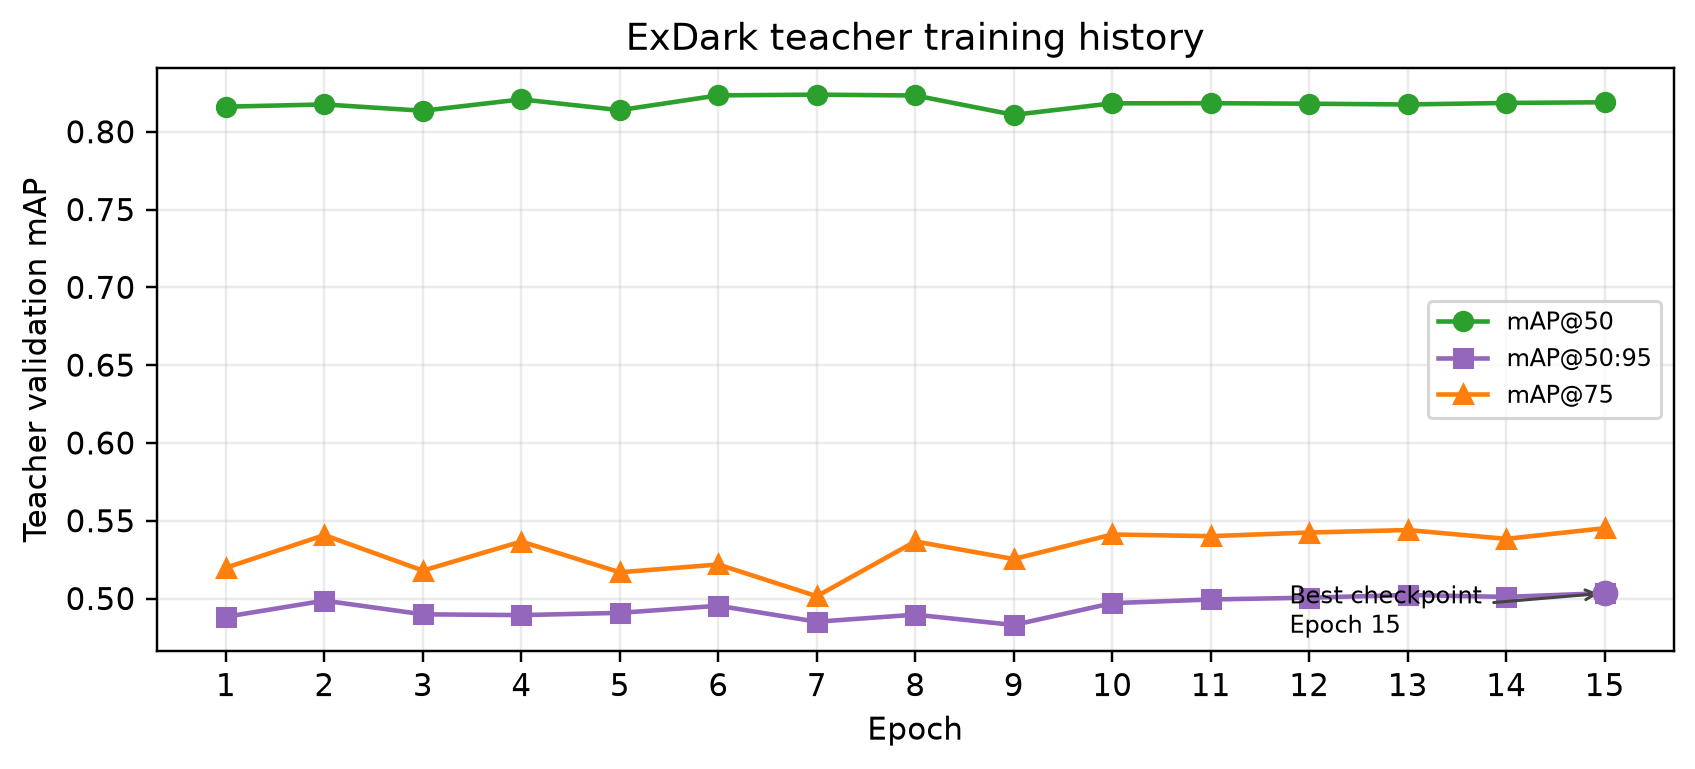
\includegraphics[width=\columnwidth]{fig/exdark_teacher_history.png}
\caption{ExDark Faster R-CNN teacher validation history across 15 epochs.
The epoch-15 checkpoint is selected by mAP@50:95.}
\label{fig:exdark_teacher_history}
\end{figure}

\subsection{Matched restoration objective}

For a low-light input \(x\), reference \(y\), and restored output
\(\hat y=F_\theta(x)\), both arms minimize
\[
L_{\mathrm{restoration}}
=
L_1(\hat y,y)
+
0.10L_{\mathrm{LPIPS}}(\hat y,y)
+
0.05L_{\mathrm{edge}}(\hat y,y).
\]
The L1 term measures RGB pixel differences. The LPIPS term uses a frozen
AlexNet perceptual network, with LPIPS inputs normalized to the
\([-1,1]\) range. The edge term uses Sobel gradients computed on the RGB
channels. The control objective contains no detection term:
\[
L_{\mathrm{control}}=L_{\mathrm{restoration}}.
\]

The control and detection-guided arms therefore receive identical
restoration supervision.

\subsection{ExDark teacher}

The detection-guided arm adds direct supervision from a frozen
ExDark-trained Faster R-CNN ResNet-50 FPN. The teacher predicts 13 outputs:
12 ExDark classes plus background. The class order is Bicycle, Boat,
Bottle, Bus, Car, Cat, Chair, Cup, Dog, Motorbike, People, and Table.

The teacher is initialized from torchvision COCO weights and transferred
to the 13-output ExDark predictor head. Matching COCO classification and
box-regression rows are copied to the corresponding ExDark categories.
The teacher is trained for 15 epochs on 2,099 ExDark teacher-training
images with 7,275 annotated boxes. The 300-image teacher-validation split,
containing 913 boxes, is used for checkpoint selection.

At epoch 15, the teacher achieves mAP@50 0.8189, mAP@50:95 0.5035, and
mAP@75 0.5452 on teacher validation. This is separate from the final
1,800-image official ExDark-validation evaluation. The best checkpoint is
stored as \texttt{models/exdark\_teacher\_v2/best.pt}.

During Balanced V2, the teacher parameters remain frozen. Detection
supervision uses the reserved 600-image ExDark detection-supervision
partition with 2,193 boxes. It does not use the teacher-validation or
official ExDark-validation partition for guidance.

\subsection{Detection-loss supervision}

For a detection-guided training step, a 640-pixel maximum-side ExDark image
is restored by DarkIR and supplied to the teacher with ground-truth boxes
and labels. The teacher returns
\[
L_{\mathrm{detector}}
=
L_{\mathrm{classifier}}
+
L_{\mathrm{box\_reg}}
+
L_{\mathrm{objectness}}
+
L_{\mathrm{RPN\_box\_reg}}.
\]
The complete detection-guided objective is
\[
L_{\mathrm{V2}}
=
L_{\mathrm{restoration}}
+
\lambda_{\mathrm{det}}L_{\mathrm{detector}}.
\]
Detection weights of 0.05, 0.10, and 0.20 are evaluated. The 0.10 model is
the primary model.

\subsection{Frozen-teacher gradient flow}

The teacher parameters remain frozen. Gradients from the four detection
losses propagate through the teacher and the restored ExDark image into
DarkIR, and only DarkIR parameters receive optimizer updates. BatchNorm
modules in the teacher are held in evaluation mode while the detector as a
whole is in training mode to obtain Faster R-CNN loss dictionaries.

The teacher uses a score threshold of 0.001 and limits retained detections
to 100 per image. Training logs verify zero teacher parameter gradients
throughout detection-guided training.

\subsection{Training configuration}

The final 5K experiments use 5,000 optimizer steps, batch size 2,
256-by-256 random LOLBlur crops, AdamW~\cite{loshchilov2019adamw} with weight decay \(10^{-4}\),
initial learning rate \(10^{-5}\), cosine decay to \(10^{-6}\), random seed
2026, and global gradient-norm clipping at 1.0. Intermediate checkpoints
are saved every 1,000 steps and final checkpoints at 5,000 steps.

Each optimizer step uses a paired LOLBlur batch for restoration
supervision and, in detection mode, one ExDark detection-supervision image.
The memory-safe implementation backpropagates the restoration and
detection branches separately, accumulating gradients in DarkIR before the
optimizer step. It does not alter the mathematical objective.

\subsection{Method scope}

The direct controlled variables are the presence of detection supervision
and the detection-loss weight. Initialization, restoration losses,
LOLBlur training data, ExDark guidance set, step count, optimizer,
scheduler, seed, and DarkIR architecture remain matched.

Balanced V2 does not implement adaptive feature modulation, joint
restoration-and-detector fine-tuning, a trainable detector head, direct
V1 feature-consistency supervision, or a change to the deployed DarkIR
architecture. It is therefore loss-level task-aware detection guidance
with a frozen ExDark-trained teacher.

\section{Datasets and Experimental Setup}
\label{sec:datasets}

\subsection{LOLBlur}

LOLBlur~\cite{zhou2022lednet} is the primary paired restoration benchmark.
The project uses the
official low-light, noisy, and blurred training set and a scene-disjoint
internal validation partition.
\begin{itemize}
  \item 9,180 training pairs and 153 training scenes.
  \item 1,020 internal-validation pairs and 17 validation scenes.
  \item Zero scene overlap between training and validation.
\end{itemize}

Each training pair contains a low-light, blurred image and a sharp,
well-exposed reference. Training uses random 256-by-256 crops and paired
horizontal and vertical flips. Full-resolution paired inference is used
for internal LOLBlur restoration validation.

\subsection{ExDark dataset partitions}

ExDark contains real low-light images annotated with 12 object categories:
Bicycle, Boat, Bottle, Bus, Car, Cat, Chair, Cup, Dog, Motorbike, People,
and Table~\cite{loh2019exdark}. The official archive contains 3,000 labeled
training images and 1,800 official-validation images.

The official training archive contains 3,000 image records. One image is
excluded because its annotation file contains no parseable bounding box.
The remaining 2,999 eligible annotated images are divided into:
\begin{itemize}
  \item 2,099 teacher-training images with 7,275 boxes.
  \item 300 teacher-validation images with 913 boxes.
  \item 600 detection-supervision images with 2,193 boxes.
\end{itemize}

The official ExDark validation partition contains 1,800 images and 6,212
ground-truth boxes. The partitions use contiguous label IDs from 1 to 12.
Image indexing excludes macOS sidecar files, and the dataset audit verifies
annotation bounds and split separation.

\begin{figure}[t]
\centering
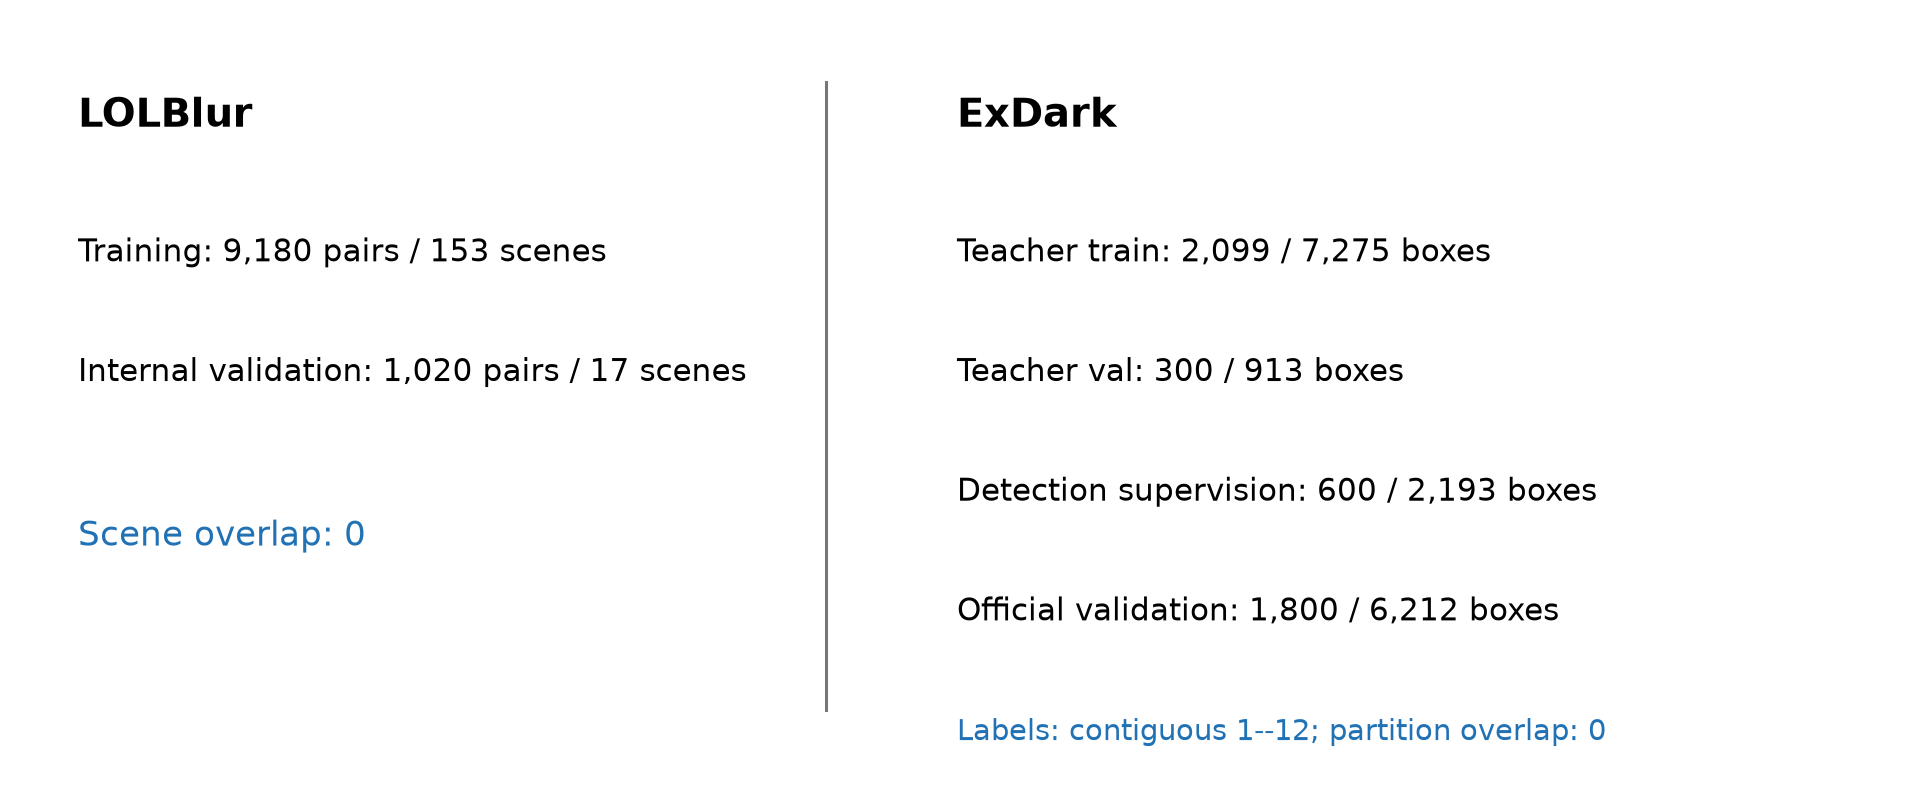
\includegraphics[width=\columnwidth]{fig/dataset_partitions.png}
\caption{Balanced V2 dataset partitions. LOLBlur training and internal
validation are scene-disjoint; ExDark teacher, guidance, and official
validation partitions remain separate.}
\label{fig:dataset_partitions}
\end{figure}

\subsection{Training configuration}

Both Balanced V2 arms initialize DarkIR-m from the pretrained checkpoint
and train for 5,000 optimizer steps. The shared configuration is:
\begin{itemize}
  \item batch size 2;
  \item LOLBlur crop size 256;
  \item AdamW optimizer;
  \item weight decay \(10^{-4}\);
  \item initial learning rate \(10^{-5}\);
  \item cosine decay to \(10^{-6}\);
  \item random seed 2026;
  \item global gradient-norm clipping at 1.0;
  \item intermediate checkpoints every 1,000 steps;
  \item final checkpoints at 5,000 steps.
\end{itemize}

The control and detection-guided arms use the same LOLBlur sample and
reference data. Detection-guided training additionally consumes one ExDark
detection-supervision image per step. ExDark images are resized so their
longest side is at most 640 pixels, and ground-truth boxes are scaled
consistently.

\subsection{Restoration evaluation}

LOLBlur internal validation reports PSNR, SSIM, and AlexNet
LPIPS~\cite{zhang2018lpips}. The SSIM protocol uses an 11-by-11 Gaussian
window, sigma 1.5, and data range 1. The LPIPS protocol uses AlexNet
features and RGB inputs normalized to \([-1,1]\). All metrics are
aggregated as macro means across the 1,020 paired validation images.

\subsection{ExDark-trained-teacher evaluation}

The first ExDark protocol uses the frozen ExDark-trained teacher:
\begin{itemize}
  \item 1,800 official-validation images;
  \item maximum side 640;
  \item score threshold 0.001;
  \item 100 detections per image;
  \item bounding-box COCOeval;
  \item IoU thresholds from 0.50 to 0.95 in 0.05 increments;
  \item 101 recall thresholds;
  \item maxDets \([1,10,100]\).
\end{itemize}

This evaluator measures original low-light inputs, V2-Control, and
V2-Detection under the same 12-class teacher.

\subsection{Independent COCO-detector evaluation}

The second ExDark protocol uses a separate frozen torchvision Faster R-CNN
ResNet-50 FPN pretrained on COCO:
\begin{itemize}
  \item 1,800 official-validation images;
  \item maximum side 640;
  \item score threshold 0.001;
  \item 100 detections per image;
  \item the same ExDark-to-COCO class mapping;
  \item the same COCOeval protocol.
\end{itemize}

This evaluator includes original low-light images, pretrained DarkIR,
V2-Control, and V2-Detection. It is independent of the ExDark-trained
guidance teacher and does not contain its ExDark fine-tuned weights.

No ExDark test images are used for model selection. Only the 1,800-image
official-validation split is used for the final V2 detection tables.

\section{Results}
\label{sec:results}

\subsection{LOLBlur restoration results}

Table~\ref{tab:lolblur_v2} reports macro PSNR, SSIM, and AlexNet LPIPS
on the 1,020-pair, scene-disjoint LOLBlur internal-validation split.
Higher PSNR and SSIM and lower LPIPS indicate better restoration.

\begin{table}[t]
\centering
\caption{Balanced V2 restoration results on 1,020 LOLBlur internal-validation pairs.}
\label{tab:lolblur_v2}
\resizebox{\columnwidth}{!}{
\begin{tabular}{lcccc}
\toprule
Model & Weight & PSNR $\uparrow$ & SSIM $\uparrow$ & LPIPS $\downarrow$ \\
\midrule
V2-Control & 0.00 & \textbf{33.5311} & \textbf{0.92083} & \textbf{0.06793} \\
V2-Detection & 0.05 & 33.4577 & 0.91982 & 0.06922 \\
V2-Detection & 0.10 & 33.4139 & 0.91929 & 0.06976 \\
V2-Detection & 0.20 & 33.3735 & 0.91863 & 0.07040 \\
\bottomrule
\end{tabular}
}
\end{table}

V2-Control achieves the best restoration metrics. Increasing the
detection-loss weight progressively decreases PSNR and SSIM and increases
LPIPS. Relative to V2-Control, the 0.10 model decreases PSNR by 0.1172 dB
and SSIM by 0.00154, while increasing LPIPS by 0.00183.

\subsection{ExDark-trained-teacher detection results}

Table~\ref{tab:exdark_teacher_v2} reports official ExDark-validation
results from the frozen ExDark-trained Faster R-CNN teacher.

\begin{table}[t]
\centering
\caption{ExDark official-validation results using the ExDark-trained guidance teacher.}
\label{tab:exdark_teacher_v2}
\resizebox{\columnwidth}{!}{
\begin{tabular}{lcccc}
\toprule
Condition & Weight & mAP@50 $\uparrow$ & mAP@50:95 $\uparrow$ & mAP@75 $\uparrow$ \\
\midrule
Original low-light & -- & \textbf{0.7501} & \textbf{0.4469} & 0.4731 \\
V2-Control & 0.00 & 0.6985 & 0.4058 & 0.4200 \\
V2-Detection & 0.05 & 0.7173 & 0.4195 & 0.4327 \\
V2-Detection & 0.10 & \textbf{0.7189} & \textbf{0.4204} & 0.4340 \\
V2-Detection & 0.20 & 0.7183 & 0.4202 & \textbf{0.4381} \\
\bottomrule
\end{tabular}
}
\end{table}

All detection-guided weights outperform V2-Control. Weight 0.10 achieves
the best mAP@50 and mAP@50:95, while weight 0.20 achieves the best mAP@75.
Original low-light images remain stronger in absolute detection
performance.

\subsection{Independent COCO-detector results}

Table~\ref{tab:coco_v2} reports the independent frozen
COCO-pretrained Faster R-CNN ResNet-50 FPN evaluation.

\begin{table}[t]
\centering
\caption{ExDark official-validation results using an independent frozen COCO-pretrained detector.}
\label{tab:coco_v2}
\resizebox{\columnwidth}{!}{
\begin{tabular}{lcccc}
\toprule
Condition & Weight & mAP@50 $\uparrow$ & mAP@50:95 $\uparrow$ & mAP@75 $\uparrow$ \\
\midrule
Original low-light & -- & \textbf{0.5869} & \textbf{0.2799} & \textbf{0.2389} \\
Pretrained DarkIR & -- & 0.5515 & 0.2635 & 0.2246 \\
V2-Control & 0.00 & 0.5530 & 0.2616 & 0.2203 \\
V2-Detection & 0.05 & 0.5730 & 0.2725 & 0.2267 \\
V2-Detection & 0.10 & \textbf{0.5753} & \textbf{0.2732} & 0.2289 \\
V2-Detection & 0.20 & 0.5722 & 0.2730 & \textbf{0.2296} \\
\bottomrule
\end{tabular}
}
\end{table}

All detection-guided conditions outperform V2-Control. Weight 0.10
achieves the best mAP@50 and mAP@50:95 among the detection-guided
configurations, and weight 0.20 is slightly better on mAP@75. Raw
low-light inputs remain the strongest absolute condition.

\begin{figure}[t]
\centering
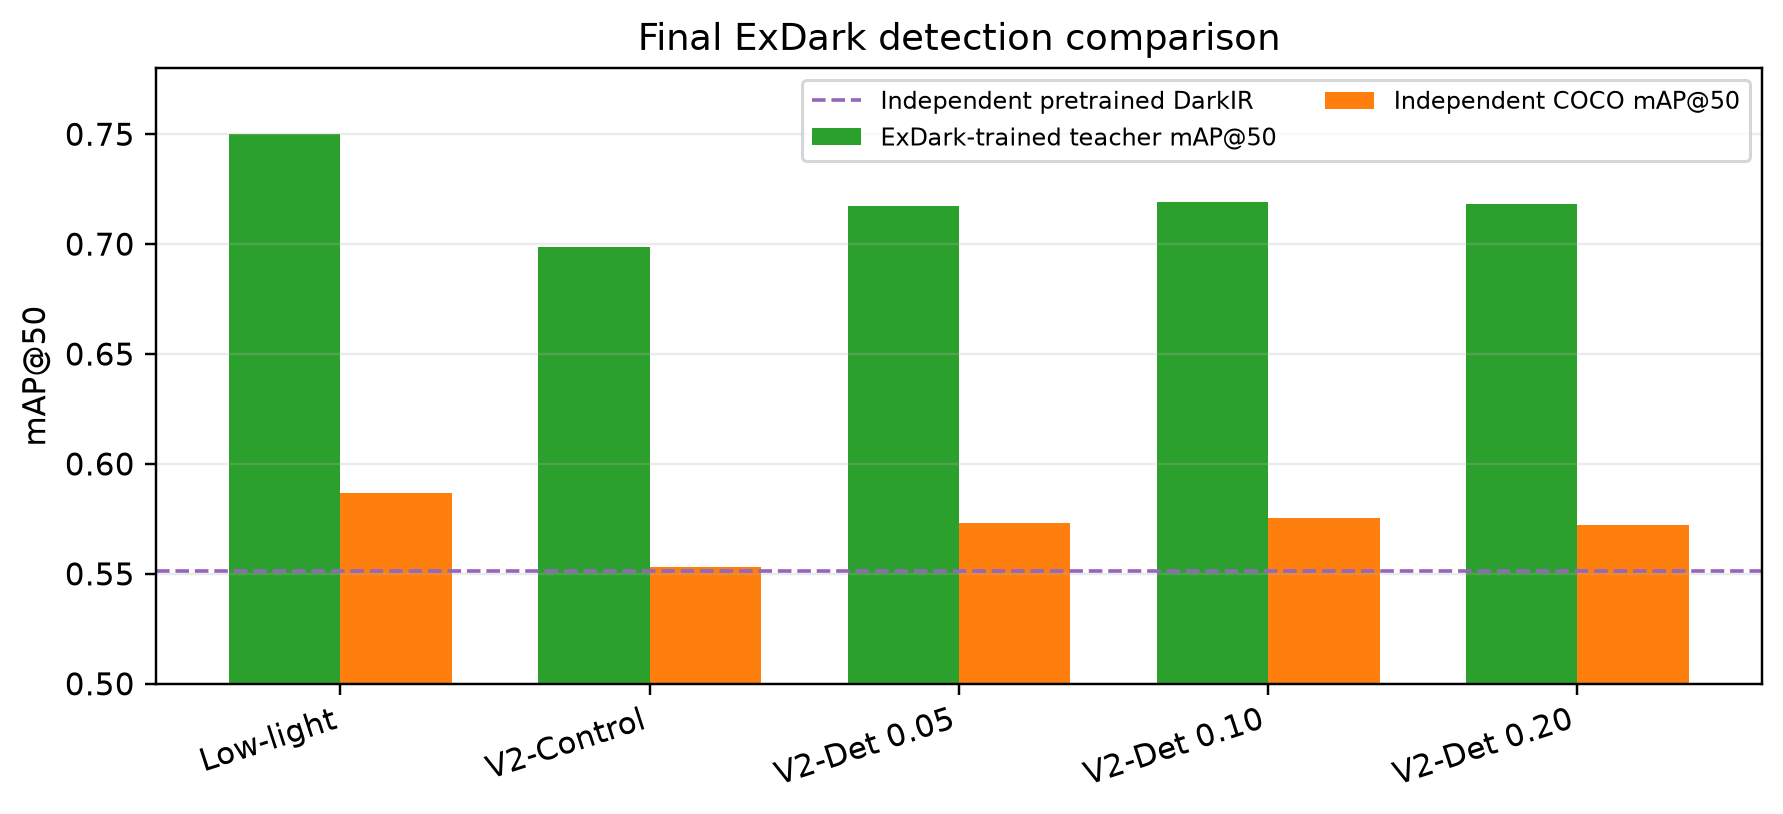
\includegraphics[width=\columnwidth]{fig/final_exdark_comparison.png}
\caption{Final mAP@50 comparison on official ExDark validation. The
ExDark-trained-teacher and independent COCO-detector protocols are shown
separately; pretrained DarkIR is included only in the independent protocol.}
\label{fig:final_exdark_comparison}
\end{figure}

To make the detector-level comparison concrete, Fig.~\ref{fig:v2_detection_overlays}
shows three illustrative official ExDark-validation examples. Each panel
uses the same original low-light photograph as a spatial backdrop. The
ground-truth boxes appear in the first column; orange boxes in the
remaining columns are predictions from the independent frozen
COCO-pretrained detector on each indicated condition, including the
pretrained model and all final V2 checkpoints. Thus, the V2 panels show
detection predictions on restored inputs, not the restored RGB outputs.

\begin{figure*}[t]
\centering
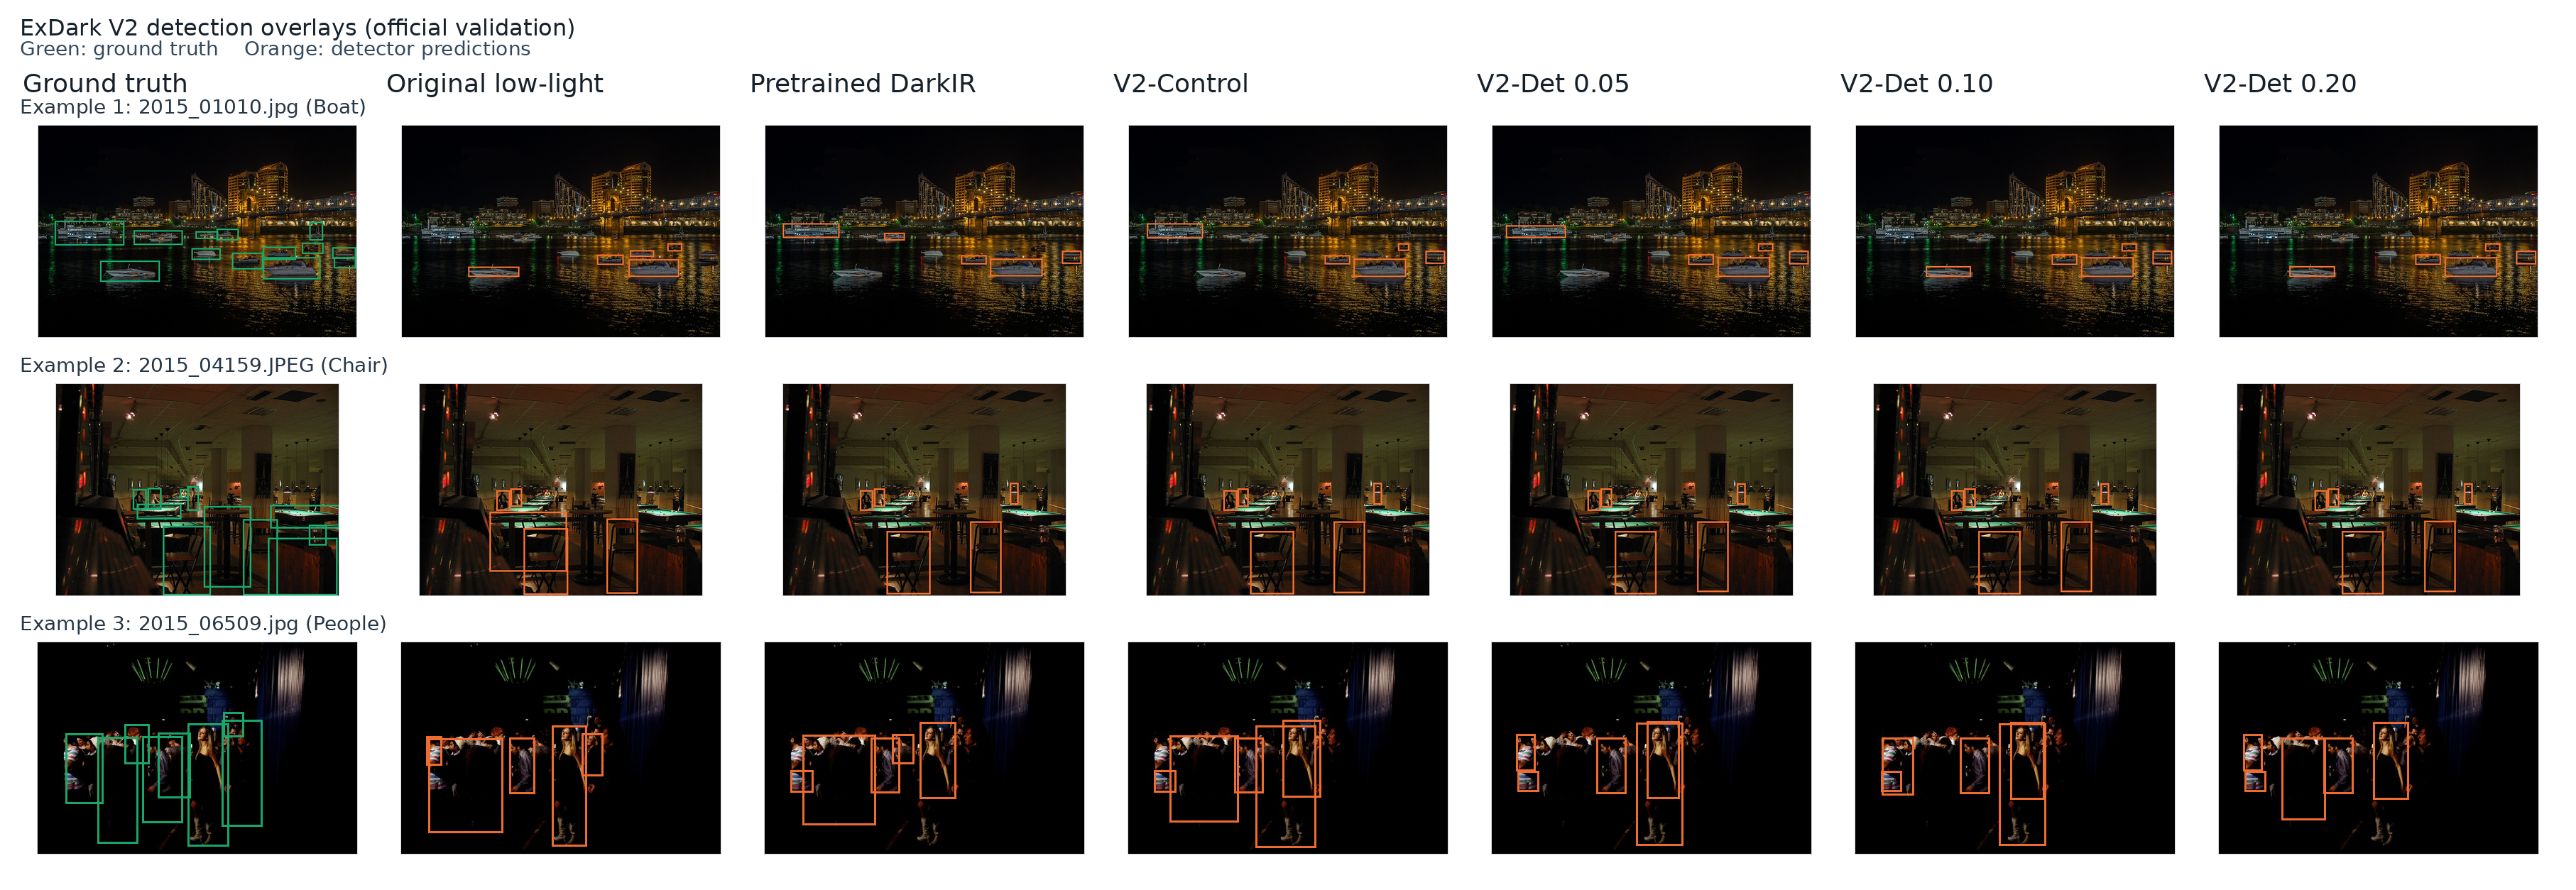
\includegraphics[width=\textwidth]{fig/v2_exdark_detection_comparison.png}
\caption{Detection overlays for three selected official ExDark-validation
images. Columns, left to right: ground truth, original low-light,
pretrained DarkIR, V2-Control, and V2-Detection weights 0.05, 0.10, and
0.20. Orange boxes show the five highest-scoring predictions from the
same independent frozen COCO-pretrained detector; panels use the original
image as a spatial backdrop. The V2 panels show detections, not restored
RGB outputs. The examples are a targeted subset: saved weight-0.10
predictions had more IoU-0.50 true-positive matches than V2-Control on
each image. They are illustrative, not random; full-validation metrics
remain the basis for quantitative comparisons.}
\label{fig:v2_detection_overlays}
\end{figure*}

\section{Detection-Weight Ablation}
\label{sec:ablation}

Table~\ref{tab:det_weight_ablation} compares the three detection-loss
weights on the 1,020-image LOLBlur restoration split and both official
ExDark-validation detectors.

\begin{table*}[t]
\centering
\caption{Detection-weight ablation for the 5K Balanced V2 detection-guided runs.}
\label{tab:det_weight_ablation}
\resizebox{\textwidth}{!}{
\begin{tabular}{lccccccccc}
\toprule
Weight & PSNR $\uparrow$ & SSIM $\uparrow$ & LPIPS $\downarrow$
& \multicolumn{3}{c}{ExDark-trained teacher}
& \multicolumn{3}{c}{Independent COCO detector} \\
\cmidrule(lr){5-7}\cmidrule(lr){8-10}
& & & & mAP@50 & mAP@50:95 & mAP@75 & mAP@50 & mAP@50:95 & mAP@75 \\
\midrule
0.05 & 33.4577 & 0.91982 & 0.06922
& 0.7173 & 0.4195 & 0.4327
& 0.5730 & 0.2725 & 0.2267 \\
0.10 & 33.4139 & 0.91929 & 0.06976
& \textbf{0.7189} & \textbf{0.4204} & 0.4340
& \textbf{0.5753} & \textbf{0.2732} & 0.2289 \\
0.20 & 33.3735 & 0.91863 & 0.07040
& 0.7183 & 0.4202 & \textbf{0.4381}
& 0.5722 & 0.2730 & \textbf{0.2296} \\
\bottomrule
\end{tabular}
}
\end{table*}

The ablation shows a consistent restoration--detection trade-off.
Weight 0.05 produces the smallest PSNR, SSIM, and LPIPS degradation
relative to V2-Control, but it has lower detection performance than
weight 0.10 under both evaluators. Weight 0.10 provides the strongest
mAP@50 and mAP@50:95 under both protocols. Weight 0.20 further degrades
restoration quality but produces the strongest mAP@75 under both
protocols.

Weight 0.10 is selected as the primary model because it is not a
simultaneous optimum for every metric, but it provides the best observed
balance between restoration and the principal mAP@50/mAP@50:95 detection
metrics. It also avoids the larger restoration penalty observed at weight
0.20.

\begin{figure}[t]
\centering
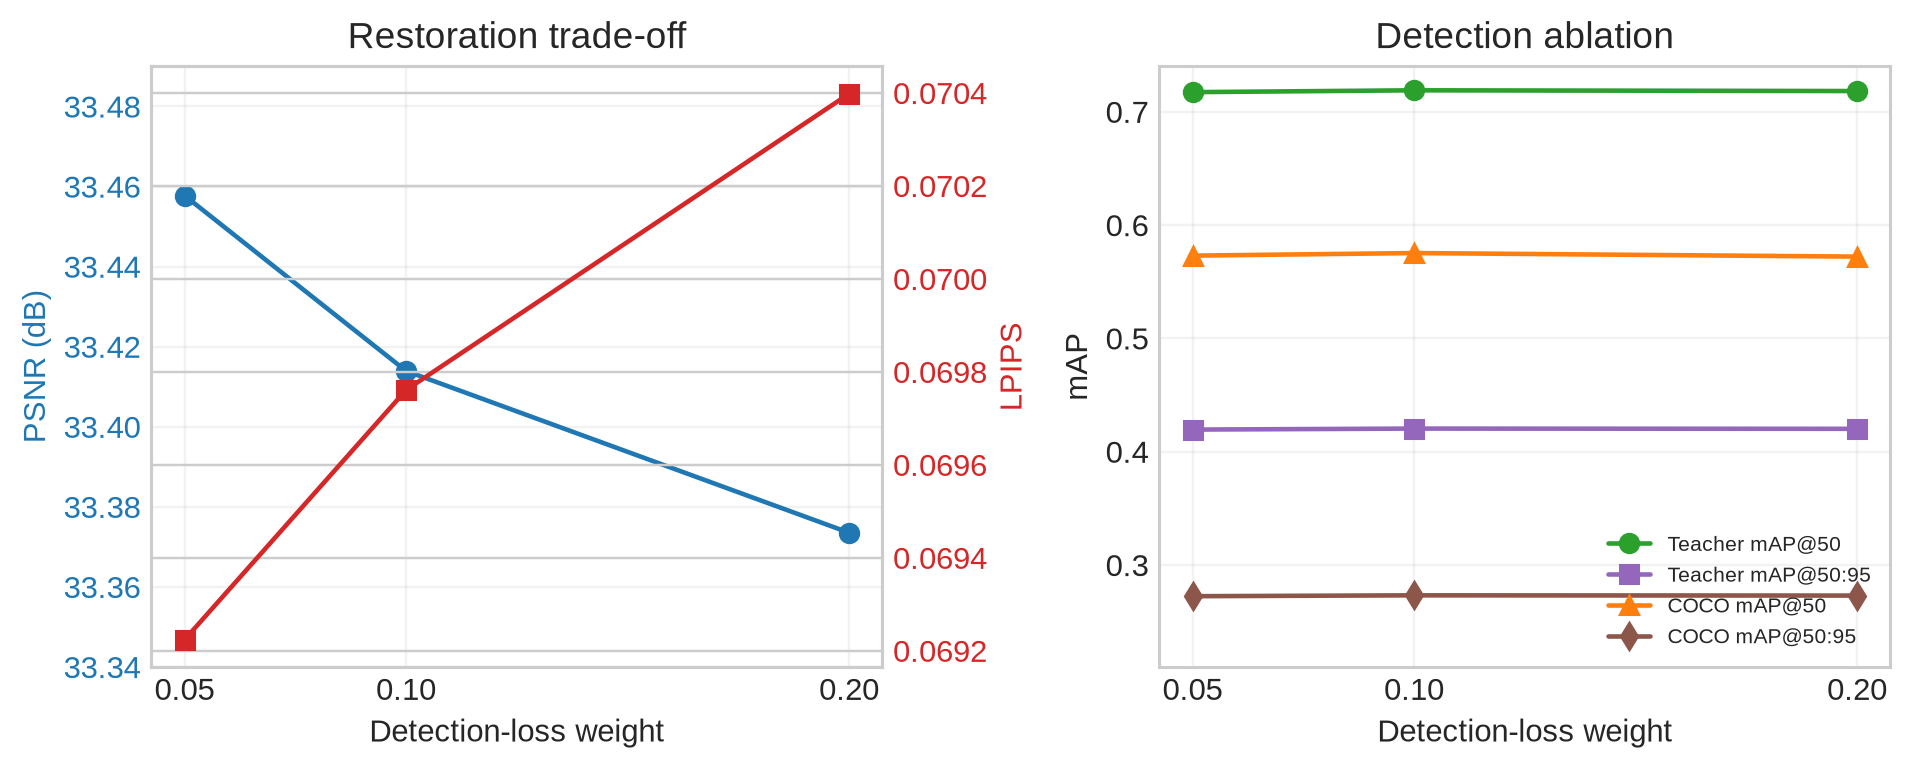
\includegraphics[width=\columnwidth]{fig/detection_weight_ablation.png}
\caption{Detection-weight ablation across restoration and detection metrics.
The 0.10 setting provides the strongest mAP@50 and mAP@50:95 balance,
while 0.20 provides the strongest mAP@75.}
\label{fig:detection_weight_ablation}
\end{figure}

\section{Per-Class Analysis}
\label{sec:per_class}

Table~\ref{tab:per_class_delta} summarizes the control-versus-detection
changes for the primary 0.10 model. Positive values indicate improvement
from V2-Control to V2-Detection.

\begin{table*}[t]
\centering
\caption{Per-class AP50 and AP50:95 differences for V2-Detection weight 0.10 relative to V2-Control.}
\label{tab:per_class_delta}
\begin{tabular}{lrrrr}
\toprule
Class & Teacher AP50 & Teacher AP50:95 & Independent AP50 & Independent AP50:95 \\
\midrule
Bicycle & +0.0083 & +0.0080 & +0.0257 & +0.0149 \\
Boat & +0.0172 & +0.0007 & +0.0098 & -0.0005 \\
Bottle & +0.0277 & +0.0136 & +0.0283 & +0.0100 \\
Bus & +0.0168 & +0.0176 & +0.0170 & +0.0180 \\
Car & +0.0226 & +0.0197 & +0.0241 & +0.0070 \\
Cat & +0.0405 & +0.0212 & +0.0476 & +0.0242 \\
Chair & +0.0134 & +0.0089 & +0.0169 & +0.0120 \\
Cup & +0.0108 & +0.0132 & +0.0133 & +0.0090 \\
Dog & +0.0208 & +0.0243 & +0.0399 & +0.0218 \\
Motorbike & +0.0433 & +0.0246 & +0.0348 & +0.0177 \\
People & +0.0174 & +0.0118 & +0.0086 & +0.0056 \\
Table & +0.0064 & +0.0120 & +0.0022 & -0.0004 \\
\bottomrule
\end{tabular}
\end{table*}

Under the ExDark-trained teacher, the 0.10 model improves both AP50 and
AP50:95 for all 12 classes relative to V2-Control. Under the independent
COCO detector, AP50 improves for all 12 classes. Independent AP50:95
improves for 10 of 12 classes, with small negative differences for Boat
and Table.

The largest independent AP50 gains occur for Cat (+0.0476), Dog
(+0.0399), Motorbike (+0.0348), and Bottle (+0.0283). The negative
independent AP50:95 changes are approximately -0.0005 for Boat and
-0.0004 for Table, while the corresponding teacher results remain positive.
Thus, aggregate detection gains vary by class and metric.

\begin{figure}[t]
\centering
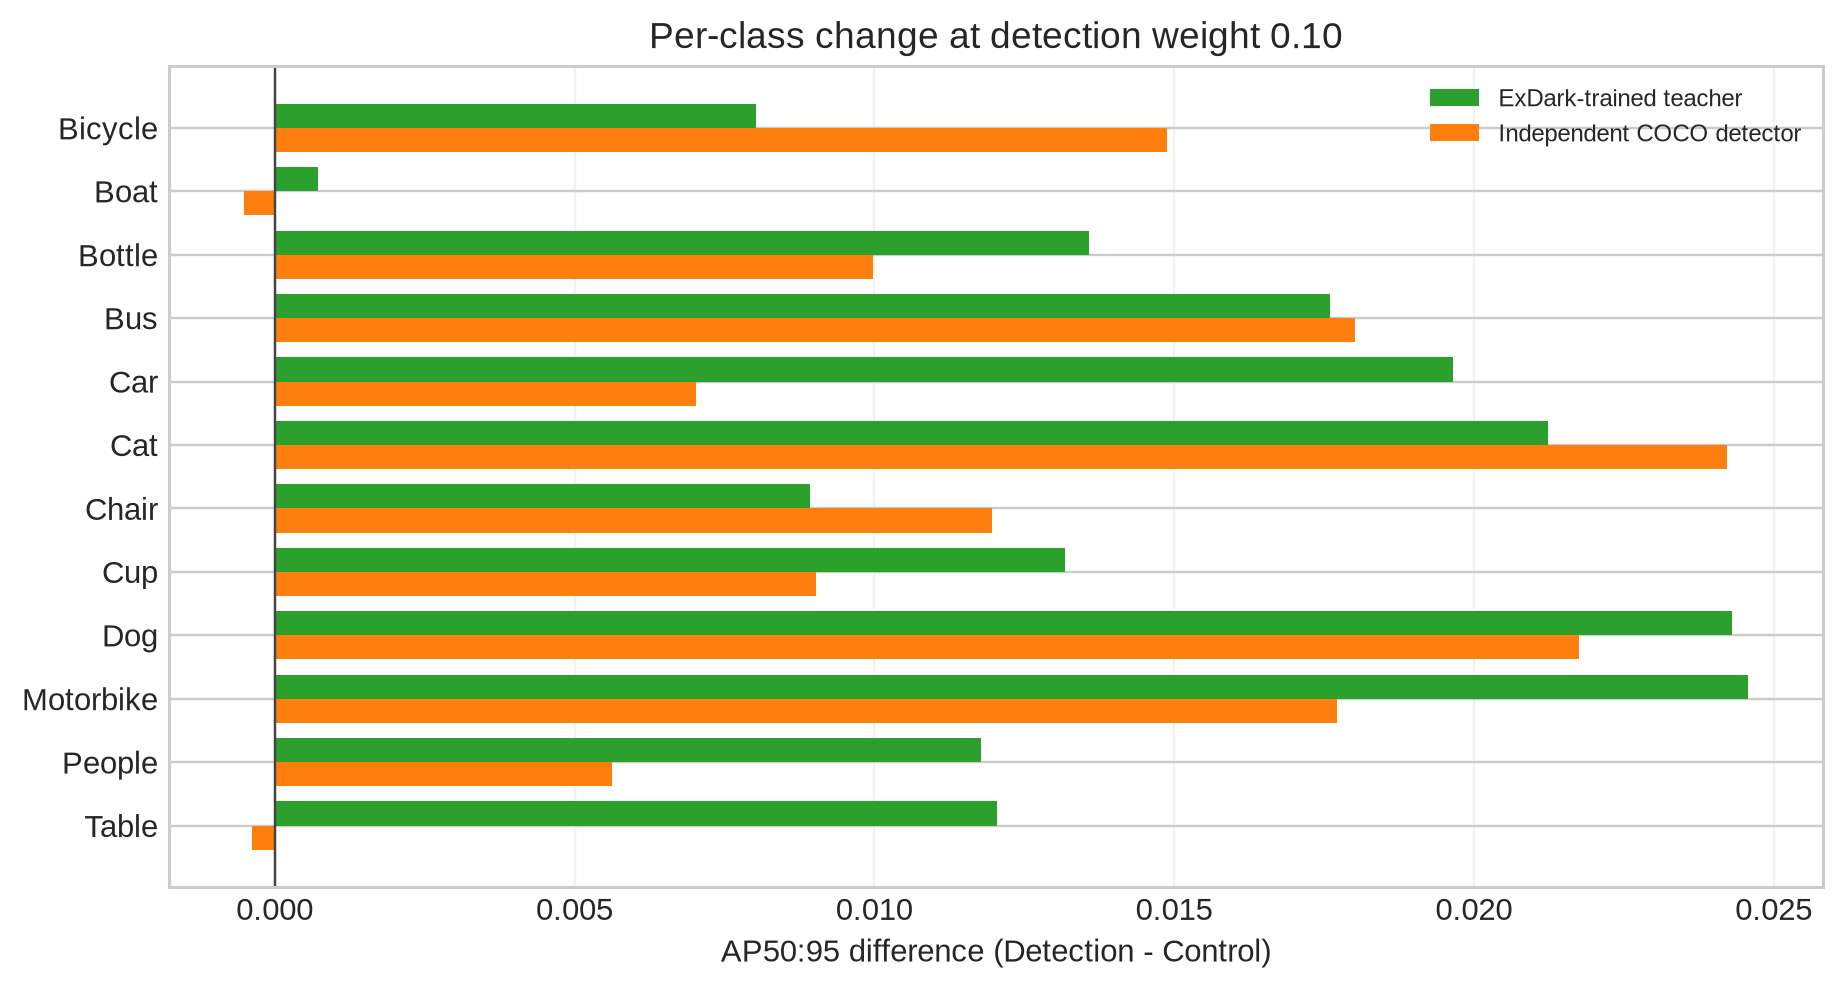
\includegraphics[width=\columnwidth]{fig/per_class_delta.png}
\caption{Control-versus-detection AP50:95 differences for weight 0.10.
Boat and Table show small negative independent-detector differences.}
\label{fig:per_class_delta}
\end{figure}

\subsection{Historical V1 and pilot evidence}

The 200-step and 1,000-step Balanced V2 pilots are development evidence
and are not used as final results. The 50,000-step V1 control and
feature-consistency experiments are historical evidence and are not
compared as if they were final Balanced V2 results.

The V1 feature-consistency model did not consistently improve detection
relative to its matched control. This negative finding motivated direct
detection-loss supervision in Balanced V2. V1 and V2 are treated as
distinct methods.

\begin{figure}[t]
\centering
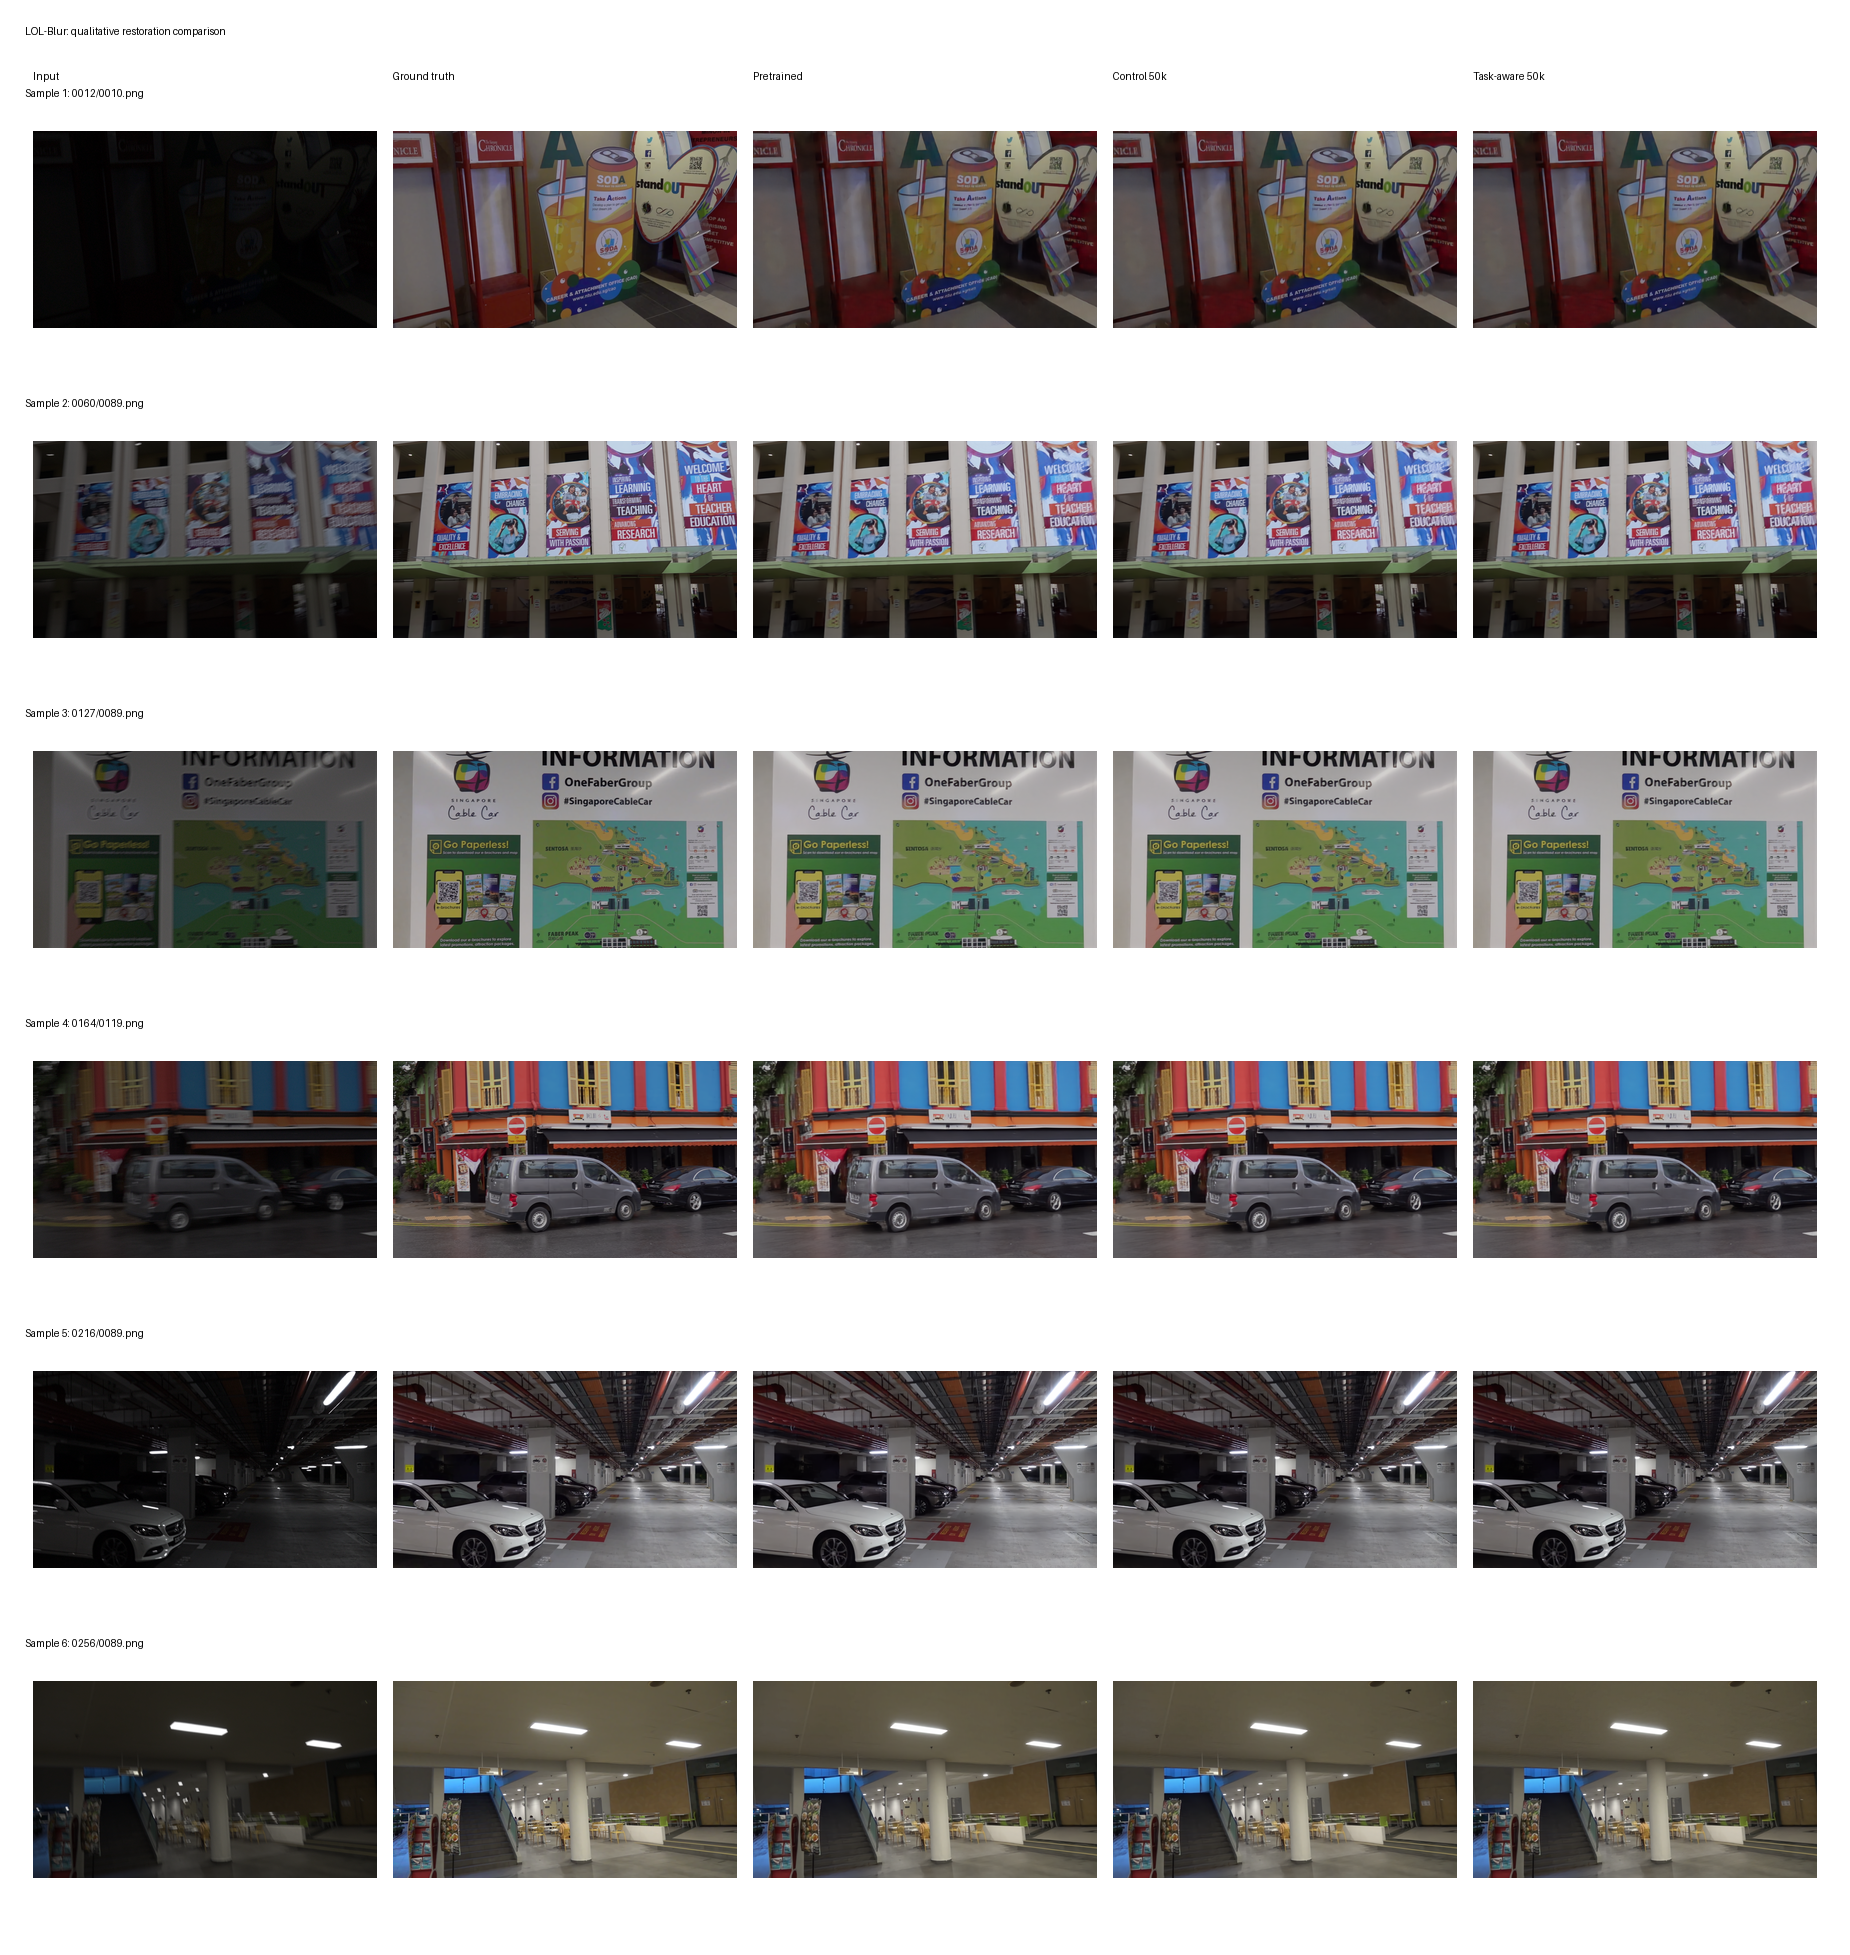
\includegraphics[width=\columnwidth]{fig/v1_qualitative_comparison.png}
\caption{Historical 50K V1 qualitative comparison. This grid is V1
feature-consistency evidence and must not be interpreted as Balanced V2
output.}
\label{fig:v1_qualitative}
\end{figure}

\section{Discussion}
\label{sec:discussion}

\subsection{Restoration--detection trade-off}

The final results demonstrate a consistent restoration--detection
trade-off in Balanced V2. Increasing the detection-loss weight improves
detection relative to V2-Control under both evaluators, but gradually
decreases PSNR and SSIM and increases LPIPS on the scene-disjoint LOLBlur
internal-validation split. The 0.10 model provides the most useful overall
balance in mAP@50 and mAP@50:95, while the 0.20 model achieves the
strongest mAP@75 but the largest restoration degradation.

This behavior indicates that image fidelity and downstream detection
utility are related but not interchangeable objectives. Detection guidance
modifies DarkIR outputs toward representations useful to the ExDark-trained
teacher, but these modifications do not uniformly maximize conventional
restoration metrics.

\subsection{V1 to V2 progression}

V1 used normalized cosine-distance features from a frozen
COCO-pretrained Faster R-CNN FPN. Reference features were evaluated
without gradients, while gradients from the restored-image feature branch
reached DarkIR. The matched 50,000-step results showed no consistent
detection improvement over the L1-only control. This negative finding
showed that matching intermediate detector features to those of a clean
reference does not necessarily improve detector decisions.

Balanced V2 replaces feature similarity with direct detection-loss
supervision. The teacher supplies classification, box-regression,
objectness, and RPN box-regression losses directly, allowing the
restoration network to optimize losses aligned more closely with the
detector objective. The matched restoration term is also expanded from
L1-only to L1, LPIPS, and Sobel edge terms.

These experiments should not be interpreted as a direct ablation where
one loss term alone explains every change, because V1 and V2 also differ
in restoration objective, dataset partitioning, teacher, step count, and
evaluation protocol. They are methodological stages with controlled
comparisons within each stage.

\subsection{Comparison with original low-light images}

The original low-light inputs remain stronger than all restored conditions
in absolute detection scores under both evaluators. Under the
ExDark-trained teacher, low-light images achieve mAP@50 0.7501 and
mAP@50:95 0.4469, compared with 0.7189 and 0.4204 for the primary 0.10
model. Under the independent COCO-pretrained detector, low-light images
achieve 0.5869 and 0.2799, compared with 0.5753 and 0.2732 for the 0.10
model.

Therefore, the project establishes improvement over V2-Control rather than
a universal benefit from restoration. Enhancement can provide a more
favorable detector input while still remaining below the original
low-light input under this evaluation protocol.

\subsection{Per-class interpretation}

The ExDark-trained-teacher evaluation improves both AP50 and AP50:95 for
all 12 classes in the primary 0.10 model. The independent detector
improves AP50 for all 12 classes and AP50:95 for 10 of 12 classes. Boat
and Table show small negative AP50:95 differences.

The per-class exceptions indicate that detection guidance is not guaranteed
to benefit every category. The aggregate gain should not be interpreted as
uniform improvement across class frequency, scale, or appearance.

\subsection{Detection-weight interpretation}

Weight 0.05 is the least restoration penalty but does not obtain the
strongest detection gain among guided models. Weight 0.10 provides the
best mAP@50 and mAP@50:95 balance under both evaluators. Weight 0.20
obtains the strongest mAP@75 but further reduces restoration quality.

The selected weight of 0.10 is therefore a trade-off choice, not a result
that maximizes every metric. The 0.20 setting may be preferable if
high-threshold localization, represented by mAP@75, is the main priority.

\subsection{Evaluator interpretation}

The ExDark-trained teacher is used for both guidance and evaluation.
It is fixed during V2 training and has been trained on ExDark. The
independent COCO-pretrained detector is not trained on ExDark and provides
a separate generalization check.

The two protocols must not be interpreted as directly comparable absolute
benchmarks. Their absolute scores differ because they use distinct
detectors, category mappings, training domains, and teacher-adaptation
histories. They support the consistent within-protocol conclusion that
detection guidance improves over V2-Control.

\section{Limitations}
\label{sec:limitations}

\subsection{Training and evaluation limitations}

Only one training seed, 2026, was used for the final Balanced V2 runs.
No multi-seed confidence intervals or statistical-significance tests are
available, so differences between control and detection-guided models
must be interpreted as measured observations rather than statistically
established gains.

The ExDark official-validation split contains 1,800 images and 6,212
ground-truth boxes. This split is used for final V2 detection evaluation
and model-weight selection. It is an official validation partition, not a
separate test set.

\subsection{Method scope}

Adaptive feature modulation was proposed in the PPR but was not implemented
or evaluated. The final study does not include the PPR B2 or B3
adaptive-modulation ablations.

Balanced V2 does not fine-tune the ExDark or COCO detectors jointly with
DarkIR. The ExDark teacher remains frozen during detection-guided
restoration training. The independent COCO-pretrained detector is also
frozen and used only for evaluation.

The final Balanced V2 restoration objective uses L1, LPIPS, and Sobel edge
losses rather than the complete DarkIR original training objective.
Therefore, the 5K fine-tuned models are not direct reproductions of the
DarkIR training recipe.

\subsection{Model and dataset scope}

The final restoration experiments are limited to DarkIR-m, width 32.
DarkIR-l and alternative restoration architectures are not compared in
the final 5K study.

The final detection supervision and evaluation use ExDark. LOLBlur is used
only for paired restoration training and internal validation. No final
cross-dataset robustness study is completed across LSRW, LOLv2,
Real-LOLBlur or illumination-stratified ExDark conditions.

\subsection{Efficiency and deployment}

Inference latency, peak GPU memory and end-to-end deployment efficiency
are not established by the core 5K experiments. The 0.338--0.339-second
detection-training step time is a training-time measurement and does not
describe deployed DarkIR inference speed.

\subsection{Pilot and historical evidence}

The 200-step and 1,000-step Balanced V2 pilots are superseded development
evidence. The earlier V1 50,000-step feature-consistency experiments are
also historical. These pilots and V1 checkpoints must not be presented as
final Balanced V2 results.

The LOLBlur test split was used during earlier baseline reproduction and
exploratory V1 development. It is therefore not presented here as an
untouched final test set.

\subsection{Qualitative and failure analysis}

The report includes a V2 detector-overlay comparison in
Fig.~\ref{fig:v2_detection_overlays}, but it does not show restored RGB
outputs from the V2 checkpoints or provide a systematic failure-case
analysis. The historical V1 restoration grid in
Fig.~\ref{fig:v1_qualitative} must not be interpreted as Balanced V2
restoration evidence.

\subsection{Interpretation limits}

Detection guidance improves over V2-Control under both evaluators, but raw
low-light inputs remain stronger in absolute detection scores. The results
therefore do not establish that restoration universally improves detection.

Per-class gains are not uniform in every metric: the independent detector
decreases Boat and Table AP50:95 slightly. Aggregate gains do not imply
that every object category or every detection threshold improves.

No claim is made that the 0.10 model is statistically optimal. It is
selected because it provides the best observed mAP@50 and mAP@50:95 balance
among the tested weights, with a smaller restoration trade-off than weight
0.20.

\section{Individual Team Contributions}
\label{sec:contributions}

The project work is divided approximately equally among the three team
members:
\begin{itemize}
  \item \textbf{Machi Reddy Hemanth Sai (33\%).}
  Responsible for the DarkIR baseline restoration work, V1 and Balanced V2
  fine-tuning development, frozen-teacher training integration, loss
  implementation, 5K checkpoint verification, and qualitative and
  quantitative visualization preparation.

  \item \textbf{N. Bhanu Prakash (33\%).}
  Responsible for dataset manifests and partition auditing, LOLBlur and
  ExDark data preparation, ExDark-trained-teacher and independent
  COCO-detector evaluator review, checkpoint verification, metric
  reconciliation, per-class analysis, and result reproducibility checks.

  \item \textbf{K. Sanjay Naidu (34\%).}
  Responsible for ExDark Faster R-CNN teacher training, teacher checkpoint
  selection and interpretation, review of both evaluator protocols,
  PPR-to-MTR-to-V1-to-V2 research narrative, equations and methodology
  synthesis, results and limitations analysis, literature review,
  conclusions and reproducibility documentation.
\end{itemize}

The Git repository history records Hemanth as the account that committed
the completed project implementation. This historical commit evidence is
separate from the final team contribution statement, which assigns
reporting and submission responsibilities across all three members.

\section{Conclusion and Future Work}
\label{sec:conclusion}

This project investigated whether task-aware low-light restoration can
improve downstream object detection while maintaining competitive image
restoration quality. The PPR proposed a feature-guided research direction,
and the MTR documented V1, a frozen-detector FPN feature-consistency
experiment. The 50,000-step V1 control and task-aware runs did not show a
consistent detection improvement, motivating a redesigned direct
detection-loss formulation.

In Balanced V2, DarkIR-m was fine-tuned from the pretrained checkpoint
using a matched L1, LPIPS, and Sobel edge restoration objective. Detection
guidance was supplied by a frozen ExDark-trained Faster R-CNN ResNet-50
FPN. The detection-guided objective added the four Faster R-CNN detection
losses with weights 0.05, 0.10, and 0.20.

The 5K experiments show that detection guidance improves over V2-Control
under both ExDark-trained-teacher and independent COCO-pretrained detector
evaluations. The primary 0.10 model achieves the strongest balance in
mAP@50 and mAP@50:95 among the guided configurations. It achieves
mAP@50 0.7189 and mAP@50:95 0.4204 under the ExDark-trained teacher, and
mAP@50 0.5753 and mAP@50:95 0.2732 under the independent COCO detector.

These detection gains come with a modest restoration-quality trade-off.
Control achieves the highest LOLBlur internal-validation PSNR, SSIM, and
lowest LPIPS. Detection weight 0.20 provides the best mAP@75 but also
the largest restoration degradation. Original low-light images remain
stronger in absolute detection scores under both evaluator protocols.

The study therefore establishes a measurable restoration--detection
trade-off, not a universal improvement from enhancement or a statistically
significant superiority claim. Its primary result is that direct
detection-loss guidance can improve a matched restoration control while
preserving the same overall restoration architecture and frozen-teacher
constraint.

Future work should evaluate multiple training seeds, a separate untouched
ExDark test split, additional detection-loss weights, full DarkIR
restoration-loss ablations, cross-dataset robustness, illumination
stratification, and restoration-only or end-to-end efficiency profiling.
Adaptive feature modulation remains a proposed future architectural
extension rather than an implemented component of Balanced V2.
